\newpage
\section{Projekt systemu wieloagentowego}

\subsection{Identyfikacja ról}

\begin{enumerate}

\item Client 
\begin{itemize}
    \item zgłasza chęć zaparkowania w pobliżu udostępnionej lokalizacji
    \item akceptuje lub odrzuca propozycje wskazanego miejsca 
\end{itemize}
 
\item Parking mapper
\begin{itemize}
    \item mapuje istniejące parkingi
\end{itemize}
\item Parking Approacher
\begin{itemize}
    \item zbliża się do parkingu i wysyła komunikat z aktualną lokalizacją
\item może zrezygnować
\end{itemize}
\item Parking Manager
\begin{itemize}
    \item kontrola dostępności miejsc na parkingu (stanu wewnętrznego),
\item przydziela miejsce parkingowe na parkingu, jeśli takie jest dostępne
\end{itemize}
\item Car Tracker 
\begin{itemize}
    \item monitoruje samochód który zarezerwował miejsce (żeby zamknąć rezerwacje jeśli
 nie będzie się zbliżał lub nie przyjedzie przez 10 min)
\end{itemize}
\end{enumerate}




\newpage
\subsection{Model ról}

\subsubsection{Parking Manager}

Aktywności:
\begin{itemize}
    \item CheckPlacesAvaliablility - sprawdzanie liczby wolnych miejsc na parkingu
    \item MakeReservation - wykonanie rezerwacji
    \item CancelReservation - zwolnienie rezerwację
\end{itemize}

Protokoły:
\begin{itemize}
    \item MapParkings
    \item PlaceReservations
    \item FreePlace
\end{itemize}


\begin{table}[!h] \label{tab:rola1} \centering
    \caption{Rola Parking Manager.}
    \begin{tabular} {| p{14cm} |} \hline
        Role schema: Parking Manager \\ \hline
        Description:

        \begin{itemize}
            \item Zwraca informacje o lokalizacji parkingu 
            \item Kontroluje dostępność miejsc na parkingu
            \item Przydziela miejsce parkingowe na danym parkingu, jeśli takie jest dostępne
            
        \end{itemize} \\ \hline
        Protocols and Activities: 
        
        \ul{CheckPlacesAvailability}, \ul{MakeReservation}, \ul{CancelReservation},

        MapParkings(SendCoordinates), PlaceReservations(SendAvailablePlaceInfo), FreePlace(ConfirmFreedPlace) \\ \hline
        Permissions:

        reads:

        generates:  parking\_location, free\_place\_count                                                                                        \\ \hline
        Responsibilities:

        Liveness:

        PARKING MANAGER = [MapParkings]. (\ul{CheckPlacesAvailability}. [SendAvailablePlaceInfo]. [\ul{MakeReservation}]. [\ul{CancelReservation}]. ConfirmFreedPlace)*
MAPPARKINGS = SendCoordinates

        Safety: true \\ \hline
    \end{tabular}
\end{table}

\newpage
\subsubsection{Car Tracker}

Aktywności:
\begin{itemize}
    \item ShouldMaintainReservation - podejmowanie decyzji o utrzymaniu rezerwacji (gdy Approacher się oddala/nie pojawia, podniesienie flagi ApproacherIsNotComing)
\end{itemize}

Protokoły:
\begin{itemize}
    \item TrackCarWithReservation 
    \item ReservationCancellation
    \item FreePlace 
\end{itemize}


\begin{table}[!h] \label{tab:rola1} \centering
    \caption{Rola Car Tracker.}
    \begin{tabular} {| p{14cm} |} \hline
        Role schema: Car Tracker \\ \hline
        Description:

        \begin{itemize}
            \item monitoruje samochód, który zarezerwował miejsce i podejmuje decyzję, czy należy rezerwacje zamknąć (jeśli np. samochód nie przybywa w ciągu kilku minut lub oddala się przez dłuższy czas)
        \end{itemize} \\ \hline
        Protocols and Activities: 
        
        \ul{ShouldMaintainReservation}, 
        
        TrackCarWithReservation(SubscribeForClientLocation), ReservationCancelation(ConfirmCancellation), FreePlace(RequestSetPlaceFree) \\ \hline
        Permissions:

        reads: approacher\_info, car\_location,  reservation\_cancellation, IsApproacher

        generates:  ApproacherIsNotComing, ApproacherCancelledReservation                                                                                   \\ \hline
        Responsibilities:

        Liveness: AR TRACKER = TrackCarWithReservation.[ReservationCancellation]. FreePlace

        TRACKCARWITHRESERVATION = SubscribeForClientLocation.ShouldMaintainReservation

        RESERVATIONCANCELLATION = ConfirmCancellation

        FREEPLACE = RequestSetPlaceFree        

        Safety: IsApproacher = True \\ \hline
    \end{tabular}
\end{table}

\newpage
\subsubsection{Parking Mapper}

Aktywności:
\begin{itemize}
    \item ComputeParkingList
    \item RunUpdate

\end{itemize}

Protokoły:
\begin{itemize}
    \item MapParking
\end{itemize}


\begin{table}[!h] \label{tab:rola1} \centering
    \caption{Rola Parking Mapper.}
    \begin{tabular} {| p{14cm} |} \hline
        Role schema: ParkingMapper \\ \hline
        Description:

        \begin{itemize}
            \item mapuje istniejące parkingi
        \end{itemize} \\ \hline
        Protocols and Activities: 
        
        \ul{RunUpdate}, MapParking(UpdateParkingsCoordiantes) \\ \hline
        Permissions:

        reads: parking\_location

        generates:  parking\_list                                                                                 \\ \hline
        Responsibilities:

        Liveness: PARKINGMAPPER = (RunUpdate.MapParking.ComputeParkingList)
        MAPPARKING = UpdateParkingsCooridnates 
        

        Safety:

        \hspace{5mm} adsa                                                                                                                                     \\ \hline
    \end{tabular}
\end{table}

\newpage
\subsubsection{Client}

Aktywności:
\begin{itemize}
    \item GetMyLocation - lokalizuje się
    \item ComputeParkingList - wybiera kilka parkingów z wolnymi miejscami w najbliższej

\end{itemize}

Protokoły:
\begin{itemize}
    \item PlaceReservation
\end{itemize}


\begin{table}[!h] \label{tab:rola1} \centering
    \caption{Rola Client.}
    \begin{tabular} {| p{14cm} |} \hline
        Role schema: Client \\ \hline
        Description:

        \begin{itemize}
            \item zgłasza chęć zaparkowania w pobliżu udostępnionej lokalizacji
            \item wybiera jeden z zaproponowanych parkingów lub odrzuca propozycje
            
        \end{itemize} \\ \hline
        Protocols and Activities: 
        
        \ul{GetMyLocation}, PlaceReservation(CallForParkingOffers, AcceptParkingOffer) \\ \hline
        Permissions:

        reads: parking\_list

        generates:  IsApproacher, car\_location, selected\_parking\_list \\ \hline
        Responsibilities:

        Liveness: Client = (GetMyLocation.CallForParkingOffers.[AcceptParkingOffer])*


        Safety: isApproacher = false \\ \hline
    \end{tabular}
\end{table}

\newpage
\subsubsection{Approacher}

Aktywności: brak

Protokoły:
\begin{itemize}
    \item TrackCarWithReservation
    \item Reservation Cancellation
    \item FreePlace
\end{itemize}


\begin{table}[!h] \label{tab:rola1} \centering
    \caption{Rola Approacher.}
    \begin{tabular} {| p{14cm} |} \hline
        Role schema: Approacher \\ \hline
        Description:

        \begin{itemize}
            \item ma zarezerwowane miejsce na parkingu i wysyła informację o swoim aktualnym położeniu (ciągle)
            \item może zrezygnować z zarezerwowanego miejsca
            
        \end{itemize} \\ \hline
        Protocols and Activities: 
        
        TrackCarWithReservation(SendReservationInfo, SendApproacherLocation), Reservation Cancellation(CancelClientReservation) \\ \hline
        Permissions:

        reads: IsApproacher

        generates:  reservation\_cancellation, car\_location \\ \hline
        Responsibilities:

        Liveness: 
        
        APPROACHER = TrackCarWithReservation.[ReservationCancellation]

        TRACKCARWITHRESERVATION = SendReservationInfo.(SendApproacherLocation)

        RESERVATIONCANCELLATION = CancelClientReservation
        

        Safety: isApproacher = true \\ \hline
    \end{tabular}
\end{table}

%%%%%%%%%%%%%%%%%%%%%%%%%%%%%%%%%%%%%%%%%%%%%%%%%%%%%%%%%%%%%

\newpage
\subsection{Model interakcji}

Na rysunku \ref{fig:interaction} przedstawiającym model interakcji widać, że nie posiada on żadnej roli centralnej komunikującej się bezpośrednio ze wszystkimi innymi rolami. System posiada znaczne rozproszenie ról, biorąc pod uwagę występowanie tylko dwóch typów agentów wcielających się w różne role. Wszystkie agenty wchodzą między sobą w interakcje. Każdy z agentów powinien zostać więc poprawnie zaimplementowany w celu utrzymania systemu.

\begin{figure}[h!]
    \centering 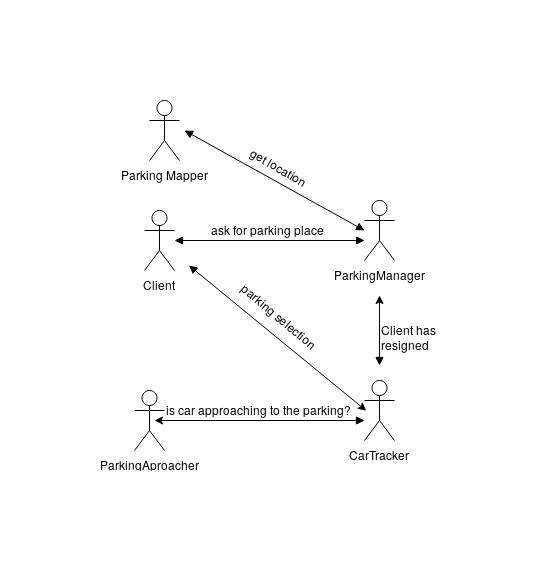
\includegraphics[width=1.0\linewidth]{interaction.png}
    \caption{Schemat interakcji.}
    \label{fig:interaction}
\end{figure}



%%%%%%%%%%%%%%%%%%%%%%%%%%%%%%%%%%%%%%%%%%%%%%%%%%%%%%%%%%%%%

\newpage
\subsection{Model agentów}

\begin{figure}[h!]
    \centering 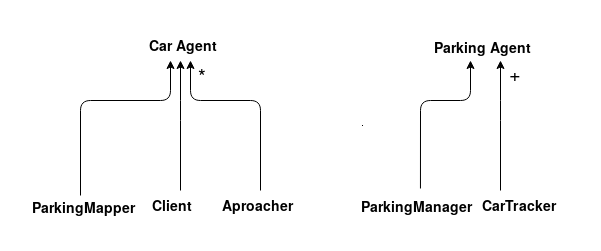
\includegraphics[width=1.0\linewidth]{agentmodel.png}
    \caption{Model agentów.}
    \label{fig:agentmodel}
\end{figure}

Na podstawie powyższych schematów (\ref{fig:agentmodel}) modeli agentów można stwierdzić, że oba rodzaje agentów  występujących w systemie są złożone w kontekście zaimplementowanych w nich ról. ParkingAgent posiada nieco większe skomplikowanie z uwagi na bardziej odpowiedzialną rolę jaką pełni w systemie, ponieważ to agenty-parkingi zarządzają agentami-pojazdami jednocześnie spełniając ich prośby. System nie może istnieć bez żadnej instancji ParkingAgent, ponieważ CarAgent w roli klienta nie mógłby wchodzić w interakcje i w rezultacie zaparkować. Natomiast można wyobrazić sobie istnienie systemu z instancjami ParkingAgent’a bez drugiego rodzaju agentów występujących w systemie.

\newpage
\subsubsection{Map Parkings}
\begin{table}[h]
    \centering
    \begin{tikzpicture}
    \node (a) at (0,0)
    {
        \begin{tabular}{|p{4cm}|p{4cm}|p{1cm}p{4cm}}
            \cline{1-2}
            \multicolumn{2}{|p{8cm}|}{UpdateParkingsCordinates (INFORM REF)} &  & \\ \cline{1-2}
            \textbf{ParkingMapper} & \textbf{ParkingManager} & \hspace{5mm}  & \\ \cline{1-3}
            \multicolumn{2}{|p{8cm}|}{Wysyła zapytania do wszystkich parkingów i uaktualnia ich położenie z prośbą o informacje o ich lokalizacji} & \hspace{5mm}  &  \\ \cline{1-3}
            \end{tabular}
    };
    \node[yshift=-2cm] (b) at (a.south) 
    {
        \begin{tabular}{|p{4cm}|p{4cm}|p{1cm}p{4cm}}
            \cline{1-2}
            \multicolumn{2}{|p{8cm}|}{SendCoordinates (INFORM)} &  & \\ \cline{1-2}
            \textbf{ParkingManager} & \textbf{ParkingMapper} & \hspace{5mm}  & \\ \cline{1-3}
            \multicolumn{2}{|p{8cm}|}{wysyła koordynaty parkingu} & \hspace{5mm}  &  parking\_location \\ \cline{1-3}
            \end{tabular}
    };
    \draw[->,ultra thick](a)--(b);
    \end{tikzpicture}
    \label{my-label}
    \end{table}

\subsubsection{PlaceReservation}
\begin{table}[h]
    \centering
    \begin{tikzpicture}
    \node (a) at (0,0)
    {
        \begin{tabular}{|p{4cm}|p{4cm}|p{1cm}p{4cm}}
            \cline{1-2}
            \multicolumn{2}{|p{8cm}|}{CallForParkingOffers (CallForProporsal)} &  & \\ \cline{1-2}
            \textbf{Client} & \textbf{Parking Manager} & \hspace{5mm}  & parking\_list \\ \cline{1-3}
            \multicolumn{2}{|p{8cm}|}{Wysyła prośbę o rezerwację miejsca postojowego do parkingów z wolnymi miejscami w określonej odległości} & \hspace{5mm}  &  \\ \cline{1-3}
            \end{tabular}
    };
    \node[yshift=-2cm] (b) at (a.south) 
    {
        \begin{tabular}{|p{4cm}|p{4cm}|p{1cm}p{4cm}}
            \cline{1-2}
            \multicolumn{2}{|p{8cm}|}{SendAvailablePlaceInfo (Propose)} &  & \\ \cline{1-2}
            \textbf{Parking Manager} & \textbf{Client} & \hspace{5mm}  &  \\ \cline{1-3}
            \multicolumn{2}{|p{8cm}|}{wysyła Clientowi informacje o dostępności miejsca, jeżeli takie posiada} & \hspace{5mm}  &  \\ \cline{1-3}
            \end{tabular}
    };
    \node[yshift=-2cm] (c) at (b.south) 
    {
        \begin{tabular}{|p{4cm}|p{4cm}|p{1cm}p{4cm}}
            \cline{1-2}
            \multicolumn{2}{|p{8cm}|}{AcceptParkingOffer (AcceptProposal)} &  & \\ \cline{1-2}
            \textbf{Client} & \textbf{Parking Manager} & \hspace{5mm}  &  \\ \cline{1-3}
            \multicolumn{2}{|p{8cm}|}{otrzymuje odpowiedź Clienta czy rezerwuje wskazane miejsce} & \hspace{5mm}  &  \\ \cline{1-3}
            \end{tabular}
    };
    \draw[->,ultra thick](a)--(b);
    \draw[->,ultra thick](b)--(c);
    \end{tikzpicture}
    \label{my-label}
    \end{table}


\newpage
\subsubsection{TrackCarWithReservation}
\begin{table}[h]
    \centering
    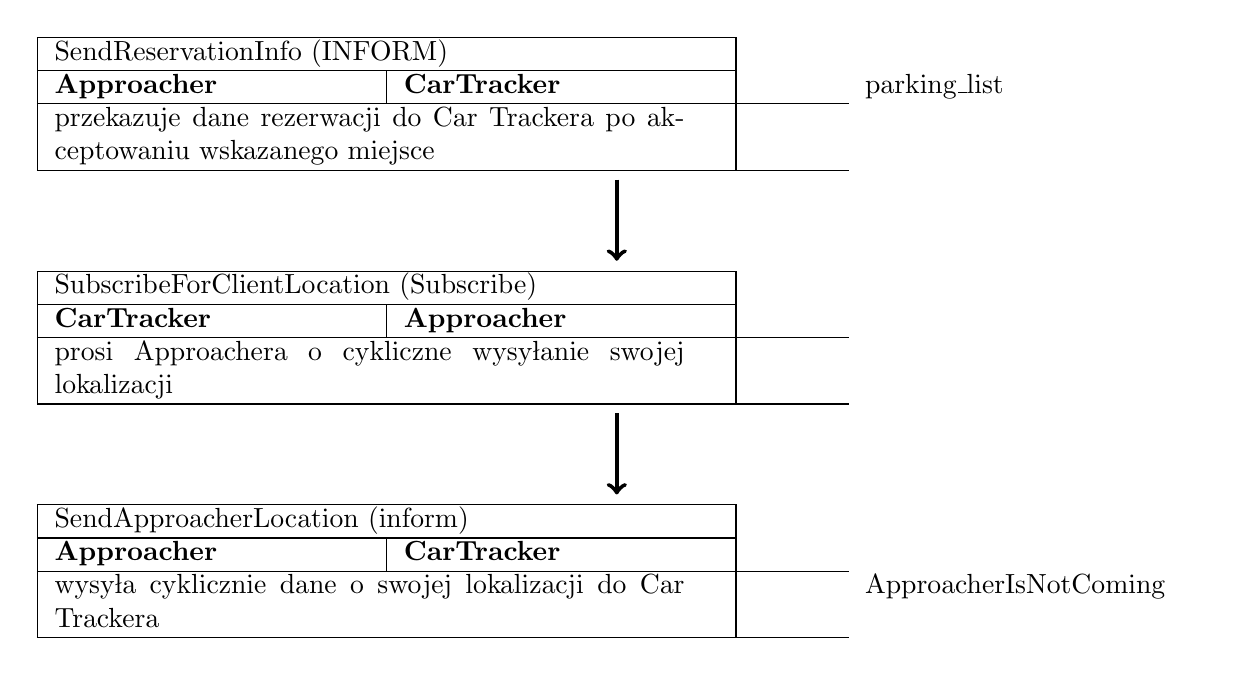
\begin{tikzpicture}
    \node (a) at (0,0)
    {
        \begin{tabular}{|p{4cm}|p{4cm}|p{1cm}p{4cm}}
            \cline{1-2}
            \multicolumn{2}{|p{8cm}|}{SendReservationInfo (INFORM)} &  & \\ \cline{1-2}
            \textbf{Approacher} & \textbf{CarTracker} & \hspace{5mm}  & parking\_list \\ \cline{1-3}
            \multicolumn{2}{|p{8cm}|}{przekazuje dane rezerwacji do Car Trackera po akceptowaniu wskazanego miejsce} & \hspace{5mm}  &  \\ \cline{1-3}
            \end{tabular}
    };
    \node[yshift=-2cm] (b) at (a.south) 
    {
        \begin{tabular}{|p{4cm}|p{4cm}|p{1cm}p{4cm}}
            \cline{1-2}
            \multicolumn{2}{|p{8cm}|}{SubscribeForClientLocation (Subscribe)} &  & \\ \cline{1-2}
            \textbf{CarTracker} & \textbf{Approacher} & \hspace{5mm}  &  \\ \cline{1-3}
            \multicolumn{2}{|p{8cm}|}{prosi Approachera o cykliczne wysyłanie swojej lokalizacji} & \hspace{5mm}  &  \\ \cline{1-3}
            \end{tabular}
    };
    \node[yshift=-2cm] (c) at (b.south) 
    {
        \begin{tabular}{|p{4cm}|p{4cm}|p{1cm}p{4cm}}
            \cline{1-2}
            \multicolumn{2}{|p{8cm}|}{SendApproacherLocation (inform)} &  & \\ \cline{1-2}
            \textbf{Approacher} & \textbf{CarTracker} & \hspace{5mm}  &  \\ \cline{1-3}
            \multicolumn{2}{|p{8cm}|}{wysyła cyklicznie dane o swojej lokalizacji do Car Trackera} & \hspace{5mm}  & ApproacherIsNotComing \\ \cline{1-3}
            \end{tabular}
    };
    \draw[->,ultra thick](a)--(b);
    \draw[->,ultra thick](b)--(c);
    \end{tikzpicture}
    \label{my-label}
    \end{table}

\subsubsection{ReservationCancellation}
\begin{table}[h]
    \centering
    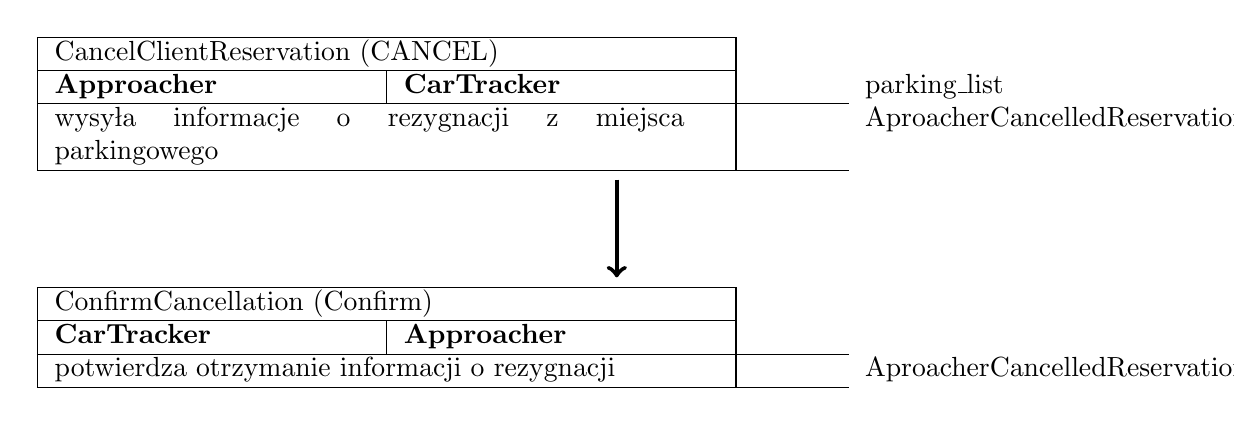
\begin{tikzpicture}
    \node (a) at (0,0)
    {
        \begin{tabular}{|p{4cm}|p{4cm}|p{1cm}p{4cm}}
            \cline{1-2}
            \multicolumn{2}{|p{8cm}|}{CancelClientReservation (CANCEL)} &  & \\ \cline{1-2}
            \textbf{Approacher} & \textbf{CarTracker} & \hspace{5mm}  & parking\_list \\ \cline{1-3}
            \multicolumn{2}{|p{8cm}|}{wysyła informacje o rezygnacji z miejsca parkingowego } & \hspace{5mm}  & AproacherCancelledReservation \\ \cline{1-3}
            \end{tabular}
    };
    \node[yshift=-2cm] (b) at (a.south) 
    {
        \begin{tabular}{|p{4cm}|p{4cm}|p{1cm}p{4cm}}
            \cline{1-2}
            \multicolumn{2}{|p{8cm}|}{ConfirmCancellation (Confirm)} &  & \\ \cline{1-2}
            \textbf{CarTracker} & \textbf{Approacher} & \hspace{5mm}  &  \\ \cline{1-3}
            \multicolumn{2}{|p{8cm}|}{potwierdza otrzymanie informacji o rezygnacji} & \hspace{5mm}  & AproacherCancelledReservation \\ \cline{1-3}
            \end{tabular}
    };
    \draw[->,ultra thick](a)--(b);
    \end{tikzpicture}
    \label{my-label}
    \end{table}


\newpage
\subsubsection{FreePlace}
\begin{table}[h]
    \centering
    \begin{tikzpicture}
    \node (a) at (0,0)
    {
        \begin{tabular}{|p{4cm}|p{4cm}|p{1cm}p{4cm}}
            \cline{1-2}
            \multicolumn{2}{|p{8cm}|}{RequestSetPlaceFree (Request)} &  & \\ \cline{1-2}
            \textbf{CarTracker} & \textbf{Parking Controller} & \hspace{5mm}  & parking\_list \\ \cline{1-3}
            \multicolumn{2}{|p{8cm}|}{wysyła żądanie usunięcia rezerwacji miejsca do Parking Controllera} & \hspace{5mm}  & \\ \cline{1-3}
            \end{tabular}
    };
    \node[yshift=-2cm] (b) at (a.south) 
    {
        \begin{tabular}{|p{4cm}|p{4cm}|p{1cm}p{4cm}}
            \cline{1-2}
            \multicolumn{2}{|p{8cm}|}{ConfirmFreedPlace (Confirm)} &  & \\ \cline{1-2}
            \textbf{Parking Controller} & \textbf{CarTracker} & \hspace{5mm}  &  \\ \cline{1-3}
            \multicolumn{2}{|p{8cm}|}{potwierdza otrzymanie informacji o rezygnacji} & \hspace{5mm}  & AproacherCancelledReservation \\ \cline{1-3}
            \end{tabular}
    };
    \draw[->,ultra thick](a)--(b);
    \end{tikzpicture}
    \label{my-label}
    \end{table}

%%%%%%%%%%%%%%%%%%%%%%%%%%%%%%%%%%%%%%%%%%%%%%%%%%%%%%%%%%%%%

\newpage
\subsection{Model usług}

\hyphenation{Approacher-Is-Not-Coming}

\begin{table}[!h] \label{tab:modeluslug} \centering
    \caption{Model usług.}
    \begin{tabular} {| m{2cm} | m{2cm} | m{3cm} | m{3cm} | m{4cm} |} \hline
        Usługa   & Wejścia & Wyjścia & Warunki wstępne & Warunki końcowe \\ \hline
        Tworzenie listy parkingów & - & parking\_list & true & parking\_list =/= NULL \\ \hline
        Znalezienie wolnego miejsca & car\_location & reservation\_info & parking\_list =/= NULL & reservation\_info =/= NULL \\ \hline
        Śledzenie położenia samochodu & car\_location reservation\_info & ApproacherIsNot\-Coming & reservation\_info =/= NULL & ApproacherIsNot\-Coming = True OR IsApproacher = False \\ \hline
        Odwoływanie zarezerwowanego miejsca & reserva\-tion\_info & Approacher\-Cancelled\-Reservation & reservation\_info =/= NULL & ApproacherCancelled\-Reservetation = True \\ \hline
    \end{tabular}
\end{table}

%%%%%%%%%%%%%%%%%%%%%%%%%%%%%%%%%%%%%%%%%%%%%%%%%%%%%%%%%%%%%


\newpage
\subsection{Model znajomości}

\begin{figure}[h!]
    \centering 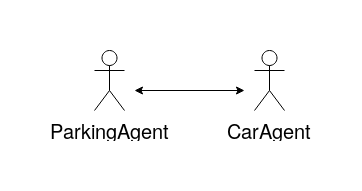
\includegraphics[width=1.0\linewidth]{friends.png}
    \caption{Model znajomości.}
    \label{fig:friends}
\end{figure}

Model znajomości agentów w systemie (Rys. \ref{fig:friends}) jest nieskomplikowany z uwagi na małą liczbę agentów w nim występujących. Wszystkie rodzaje agentów komunikują się między sobą. Nadmienić należy że architektura systemu została zaprojektowana w ten sposób, że nie wymaga komunikacji pomiędzy różnymi instancjami tego samego rodzaju agenta. W ParkingAgent następuje komunikacja pomiędzy rolami, w które wciela się ta sama instancja tego rodzaju genta.